\section{Le protocole EnOcean}

On se place dans le cas d'une chaine hôtelière souhaitant réaliser des travaux sur un bâtiment existant afin de moderniser l'éclairage, le chauffage ainsi que la climatisation de ses chambres sans faire de travaux. L'entreprise souhaite générer des économies tout en maintenant le confort des clients.

\UPSTIquestion{Selon vous, quels seraient les avantages d'une solution sans-fil et centralisée pour répondre à cette demande ?}

\subsection{Présentation}
Le protocole EnOcean est un protocole de communication sans fil. Il est utilisé pour la gestion de l'éclairage, du chauffage, de la ventilation et de la climatisation (CVC). Il est également utilisé pour la gestion des stores et des volets roulants.
Ce protocole présente les caractéristiques suivantes : 
\begin{description}
    \item[Fréquence d'émission] 868 MHz
    \item[Portée] 30 m en intérieur, 300 m en extérieur
    \item[Alimentation] par récupération d'énergie (énergie solaire, thermique, mécanique)
    \item[Nombre de participants] 65 000
    \item[Débit] 125 kbit/s 
\end{description}

Pour communiquer avec un capteur EnOcean, il nous faudra utiliser un coupleur EnOcean.  Ce coupleur communique avec un automate WAGO par un bus série RS485. Nous aurons donc besoin d'un coupleur de liaison série sur le bus de l'automate. Nous utiliserons un module WAGO 750-652 comme coupleur de liaison série.
Cette automate gérera également un éclairage DALI. 


\UPSTIquestion{Donner le schéma synoptique complet de l'installation. Vous devrez faire apparaitre : 
\begin{itemize}
    \item le capteur de température extérieure,
    \item l'automate WAGO,
    \item le coupleur EnOcean,
    \item le coupleur RS485,
    \item le coupleur DALI,
    \item un ballast DALI,
    \item un luminaire DALI.
    \item le réseau RS485.
    \item le réseau sans-fil EnOcean.
    \item le réseau DALI.
    \end{itemize}
    }

\UPSTIquestion{Le réseau Enocean peut être de type Etoile ou Maillé. Expliquer les différences entre ces deux topologies.}

\UPSTIquestion{Faire un schéma de ces deux topologies.}

\subsection{Télégramme}
Un message EnOcean est une suite de $n$ octets comprenant deux octets de synchronisation, un entête (header), des données se terminant par un octet de statut et enfin un octet de contrôle (checksum).

\begin{figure}[h!t]
    \centering
    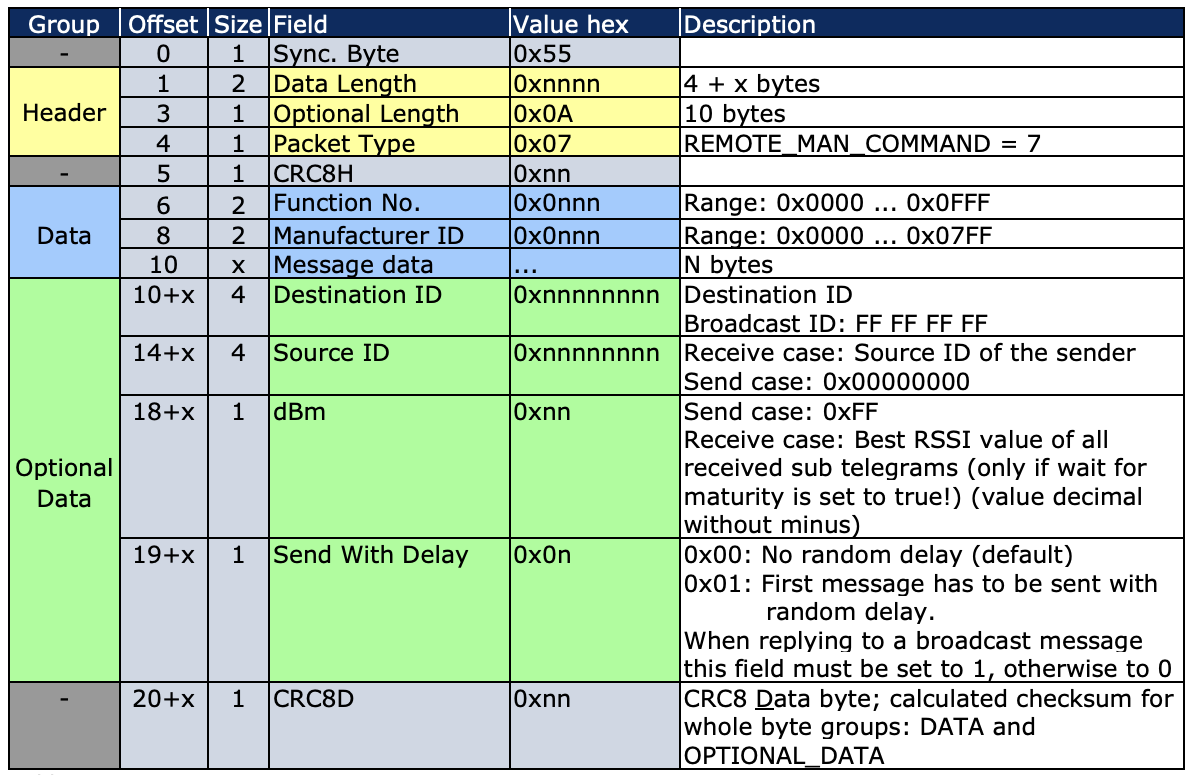
\includegraphics[width=0.67\linewidth]{telegramme.png}
    \caption{Télégramme EnOcean}
    \label{fig:telegramme}
\end{figure}

On s'intéresse ici à la mise en oeuvre d'un capteur de température extérieure EnOcean SR65 du constructeur Thermokon. Ce capteur de température a pour profil \textit{07-02-14}. Les données sont envoyées sur 7 octets.

\UPSTIquestion{A partir de l'annexe et du profil de capteur ci-dessus, Donner la valeur de l'octet correspondant au type de capteur.}


\UPSTIquestion{A partir des informations ci-dessus et de la Figure~\ref{fig:telegramme}, quelle est la taille d'un télégramme complet envoyé par ce capteur ?}
\UPSTIquestion{En déduire le temps d'émission de ce capteur lors de l'envoi d'une information de température.}


\subsection{Récupération de la température}
On donne en annexe la documentation des blocs fonctions \textbf{FbThermokonSRC65\_RS485\_EVC} et \textbf{FbA502xx\_TemperatureSensor}. 

\UPSTIquestion{Expliquer le rôle de chacun de ces deux blocs.}

\UPSTIquestion{Proposer un programme en Blocs fonctions (CFC) permettant de récupérer la valeur de la température et de la stocker dans une variable que l'on nommera \textit{r\_temperature}. Faire les déclarations nécessaires.}

\UPSTIquestion{Afin d'éviter l'éparpillement des données dans le cas où l'on multiplierait le nombre de capteurs, proposer la définition d'une classe associée au bloc fonction \textbf{FbA502xx\_TemperatureSensor}}

